% !TeX program = xelatex
% !BIB program = biber
% Hlavní dokument v Overleafu: main.tex. Kompilátor: XeLaTeX.
% ZAČNĚTE: otevřete START.md; před odevzdáním projděte KONTROLA.md.
% Orientace v editoru: vyhledejte TODO nebo název kapitoly.
% TODO označuje místo k ruční kontrole. Po vyřízení smažte jeho komentář.
% Komunitní uspořádání Adama Kábrta s využitím Codexu.
% Třída: Pavel Satrapa; výchozí místní balíček s úpravami Jana Koprnického.

%%%%%%%%%%%%%%%%%%%%%%%%%%%% PREAMBULE %%%%%%%%%%%%%%%%%%%%%%%%%%%%

% ZÁKLAD PRO SESTAVENÍ: documentclass a načtení nastavení ponechte.
% Nastavení dokumentu. Vlastní text práce začíná až v části TEXT PRÁCE.
% Balíčky: nastaveni/balicky.tex | Osobní údaje: nastaveni/udaje.tex
% TODO: potvrďte fakultu a typ práce podle zadání; FM,BP je pouze ukázka.
\documentclass[FM,BP]{tulthesis}
% Fakultu a typ práce upravte výše; toto je ukázka FM / bakalářská práce.
% Nastavení společné pro celou práci. Samotné kapitoly balíčky nenačítají.
\usepackage{polyglossia}
\setdefaultlanguage{czech}
\usepackage{csquotes}
\usepackage[backend=biber,style=iso-numeric,sorting=nyt,autolang=other,bibencoding=UTF8]{biblatex}
\addbibresource{literatura/zdroje.bib}
% Styl citací ověřte podle požadavků fakulty; ukázka nepředepisuje normu.
\DeclareFieldFormat{labelnumberwidth}{\mkbibbrackets{#1}}
% Pokud měníte cestu k obrázkům, ponechte i cestu k logům šablony.
% Společné vyhledávání obrázků a původních PDF značek všech fakult.
\graphicspath{{obrazky/}{sablona/loga/TUL/}{sablona/loga/FM/}{sablona/loga/FS/}{sablona/loga/FT/}{sablona/loga/FP/}{sablona/loga/EF/}{sablona/loga/FUA/}{sablona/loga/FZS/}{sablona/loga/CXI/}}


% Všechny údaje jsou ukázkové. Nahraďte je údaji své práce.
% Údaje přebírejte ze zadání a IS/STAG; příklady nejsou fakultní doporučení.
% Vyplňujte text uvnitř složených závorek; příkazy a počet argumentů zachovejte.
% Znak & pište jako \&, % jako \%, podtržítko jako \_.
% TODO: český a anglický název práce.
\TULtitle{Ukázková práce}{Example thesis}
% TODO: jméno autora v požadovaném tvaru.
\TULauthor{Jméno Příjmení}
% TODO: kód programu, český název, anglický název.
\TULprogramme{KÓD}{Název programu}{Programme name}
% TODO: údaje oboru a jejich použitelnost ověřte podle své fakulty.
\TULbranch{KÓD}{Název oboru}{Field of study}
% TODO: jméno a případné tituly vedoucího podle zadání.
\TULsupervisor{Jméno vedoucího}
% TODO: potvrďte rok odevzdání; ukázkový rok nemusí odpovídat vaší práci.
\TULyear{2026}



%%%%%%%%%%%%%%%%%%%%%%%%%% ÚVODNÍ ČÁSTI %%%%%%%%%%%%%%%%%%%%%%%%%%%

% DLE POKYNŮ FAKULTY: úvodní listy, abstrakty a klíčová slova.
% Zde jsou ukázkové texty; poděkování je volitelné.
% Ukázkové věty nahraďte svými; ponechte příkazy begin a end prostředí.
\begin{document}
% Prototyp generuje ukázkové úvodní strany a prohlášení v mužském rodě.
% Před odevzdáním použijte aktuální požadované listy z IS/STAG podle fakulty.
% Pokud máte jejich PDF ve složce prilohy/, nahraďte následující příkaz:
% \ThesisStart{prilohy/zadani-a-prohlaseni.pdf}
% TODO: ověřte úvodní listy; male/female jsou ukázkové varianty prohlášení.
\ThesisStart{male}

%%%%%%%%%%%% ČESKÝ ABSTRAKT A KLÍČOVÁ SLOVA %%%%%%%%%%%%

\begin{abstractCZ}
  % TODO: nahraďte ukázku vlastním českým abstraktem.
  Doplňte český abstrakt své práce. Tento dokument pouze ověřuje nové uspořádání souborů.
\end{abstractCZ}

\begin{keywordsCZ}
  % TODO: doplňte vlastní klíčová slova.
  ukázka, uspořádání projektu
\end{keywordsCZ}

%%%%%%%%%%%% ANGLICKÝ ABSTRAKT A KLÍČOVÁ SLOVA %%%%%%%%%%%%

\begin{abstractEN}
  % TODO: doplňte odpovídající anglický abstrakt.
  Replace this text with the abstract of your thesis.
\end{abstractEN}

\begin{keywordsEN}
  % TODO: doplňte anglická klíčová slova.
  example, project structure
\end{keywordsEN}

%%%%%%%%%%%% PODĚKOVÁNÍ — VOLITELNÉ %%%%%%%%%%%%

% Pokud je nechcete, smažte celé prostředí acknowledgement i jeho text.

\begin{acknowledgement}
  Doplňte poděkování nebo toto prostředí odstraňte.
\end{acknowledgement}

%%%%%%%%%%%% OBSAH — GENERUJE SE AUTOMATICKY %%%%%%%%%%%%

% Sem nic ručně nevypisujte; obsah se sestaví podle nadpisů v práci.
\tableofcontents


%%%%%%%%%%%%%%%%%%%%%%%%%%% TEXT PRÁCE %%%%%%%%%%%%%%%%%%%%%%%%%%%%%

% TADY PIŠTE VLASTNÍ TEXT. Názvy a počet kapitol přizpůsobte své práci.
% UKÁZKY K NAHRAZENÍ: věty, citace, tabulka a obrázek nejsou vaše výsledky.
% Ponechte begin{document} nahoře a end{document} na konci souboru.

%%%%%%%%%%%% 01 — ÚVOD %%%%%%%%%%%%

\chapter{Úvod}
\label{chap:uvod}
% TODO: napište vlastní úvod a nahraďte ukázkovou citaci ověřeným zdrojem.

Popište motivaci, cíl a rozsah vlastní práce. Osnova je ukázková.
Dokumentace původní šablony je uvedena jako příklad zdroje~\autocite{satrapa-manual}.

%%%%%%%%%%%% 02 — METODIKA %%%%%%%%%%%%

\chapter{Metodika}
\label{chap:metodika}
% TODO: popište vlastní postup; osnova není závazným členěním práce.

Na cíl z kapitoly~\ref{chap:uvod} navazuje zvolený postup.
Vysvětlete, jak získáte podklady a jak budete vyhodnocovat výsledky.

%%%%%%%%%%%% 03 — VÝSLEDKY A DISKUSE %%%%%%%%%%%%

\chapter{Výsledky a diskuse}
\label{chap:vysledky}
% TODO: nahraďte syntetické ukázky vlastními výsledky nebo odstraňte celé bloky.

Uveďte vlastní výsledky, jejich interpretaci a omezení. Ukázková tabulka~\ref{tab:ukazka} neobsahuje skutečné měření.
% ZAČÁTEK UKÁZKY TABULKY — tento blok lze smazat až po KONEC UKÁZKY.
% Potom upravte i větu nad ním, která na tabulku odkazuje.
\begin{table}[ht]
\centering
\caption{Syntetické hodnoty pro kontrolu sazby}
\label{tab:ukazka}
\begin{tabular}{lr}
Vzorek & Hodnota \\
A & 12,4 \\
B & 13,1
\end{tabular}
\end{table}
% KONEC UKÁZKY TABULKY

% ZAČÁTEK UKÁZKY OBRÁZKU — smažte celý blok, pokud jej nepotřebujete.
% Graf je syntetický; změna hodnot v tabulce jej nepřepočítá.
% Vlastní obrázek nahrajte do obrazky/ a změňte název v includegraphics.
\begin{figure}[ht]
  \centering
  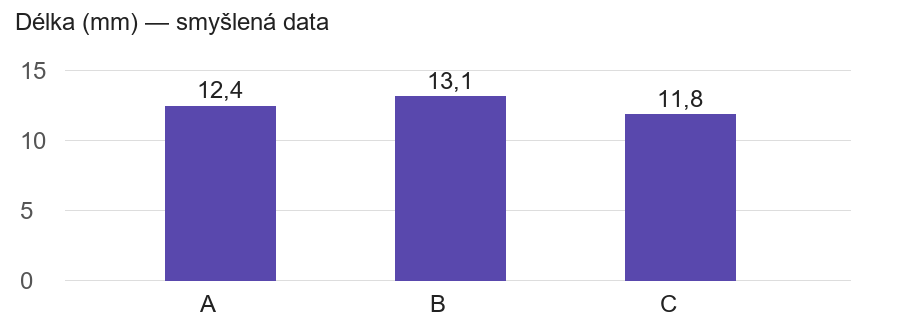
\includegraphics[width=.65\textwidth]{ukazka-mereni.png}
  \caption{Syntetický graf pro vyzkoušení obrázku}
  \label{fig:ukazka}
\end{figure}
Ukázkový obrázek~\ref{fig:ukazka} slouží pouze k ověření sazby.
% KONEC UKÁZKY OBRÁZKU — při odstranění smažte také větu s odkazem.

%%%%%%%%%%%% 04 — ZÁVĚR %%%%%%%%%%%%

\chapter{Závěr}
% TODO: nahraďte pokyn vlastním závěrem.
Shrňte splnění cíle, hlavní výsledky a možnosti další práce.


%%%%%%%%%%%%%%%%%%%%%%%%% POUŽITÁ LITERATURA %%%%%%%%%%%%%%%%%%%%%%%

% Seznam se generuje z citací a souboru literatura/zdroje.bib.
% Jednotlivé záznamy upravujte v .bib, ne za tímto příkazem.
\printbibliography[title={Použitá literatura},heading=bibintoc]

%%%%%%%%%%%%%%%%%%%%%%%%%%%%% PŘÍLOHY %%%%%%%%%%%%%%%%%%%%%%%%%%%%%%

% Sem patří textové přílohy; samostatné soubory ukládejte do prilohy/.
% Pokud přílohy nemáte, smažte celou část od appendix po poslední text.
% Poslední příkaz end{document} ale ponechte.
\appendix
\chapter{Doplňující podklady}
% TODO: doplňte vlastní přílohy nebo odstraňte celou přílohovou část.
Přidejte přílohy podle potřeb práce. Pokud přílohy nemáte, odstraňte tuto část podle komentáře výše.

%%%%%%%%%%%%%%%%%%%%%%%%% KONEC DOKUMENTU %%%%%%%%%%%%%%%%%%%%%%%%%%

\end{document}
